%!TEX root = book.tex
\chapter{Giới thiệu về Feature Engineering}
 
 
\section{Giới thiệu }
 
Cho tới lúc này, tôi đã trình bày 5 thuật toán Machine Learning cơ bản: \href{http://machinelearningcoban.com/2016/12/28/linearregression/}{Linear Regression}, \href{http://machinelearningcoban.com/2017/01/01/kmeans/}{K-means Clusterning}, \href{http://machinelearningcoban.com/2017/01/08/knn/}{K-nearest neighbors}, \href{http://machinelearningcoban.com/2017/01/21/perceptron/}{Perceptron Learning Algorithm} và \href{http://machinelearningcoban.com/2017/01/27/logisticregression/}{Logistic Regression}. Trong tất cả các thuật toán này, tôi đều giả sử các điểm dữ liệu được biểu diễn bằng các vector, được gọi là \textit{feature vector} hay \textit{vector đặc trưng}, có độ dài bằng nhau, và cùng là vector cột hoặc vector hàng. Tuy nhiên, trong các bài toán thực tế, mọi chuyện không được tốt đẹp như vậy! 
 
Với các bài toán về Computer Vision, các bức ảnh là các ma trận có kích thước khác nhau. Thậm chí để nhận dạng vật thể trong ảnh, ta cần thêm một bước nữa là \textit{object detection}, tức là tìm cái khung chứa vật thể chúng ta cần dự đoán. Ví dụ, trong bài toán nhận dạng khuôn mặt, chúng ta cần tìm được vị trí các khuôn mặt trong ảnh và \textit{crop} các khuôn mặt đó trước khi làm các bước tiếp theo. Ngay cả khi đã xác định được các khung chứa các khuôn mặt (và có thể resize các khung đó về cùng một kích thước), ta vẫn phải làm rất nhiều việc nữa vì hình ảnh của khuôn mặt còn phụ thưộc vào góc chụp, ánh sáng, ... và rất nhiều yếu tố khác nữa.  
 
Các bài toán NLP (Natural Language Processing - Xử lý ngôn ngữ tự nhiên) cũng có khó khăn tương tự khi độ dài của các văn bản là khác nhau, thậm chí có những từ rất hiếm gặp hoặc không có trong từ điển. Cũng có khi thêm một vài từ vào văn bản mà nội dung của văn bản không đổi hoặc hoàn toàn mang nghĩa ngược lại. Hoặc cùng là một câu nói nhưng tốc độ, âm giọng của mỗi người là khác nhau, thậm chí của cùng một người nhưng lúc ốm lúc khỏe cũng khác nhau.  
 
Khi làm việc với các bài toán Machine Learning thực tế, nhìn chung chúng ta chỉ có được dữ liệu thô (raw) chưa qua chỉnh sửa, chọn lọc. Chúng ta cần phải tìm một phép biến đổi để loại ra những dữ liệu nhiễu (noise), và để đưa dữ liệu thô với số chiều khác nhau về cùng một chuẩn (cùng là các vector hoặc ma trận). Dữ liệu chuẩn mới này phải đảm bảo giữ được những thông tin đặc trưng (features) cho dữ liệu thô ban đầu. Không những thế, tùy vào từng bài toán, ta cần \textit{thiết kế} những phép biến đổi để có những features phù hợp. Quá trình quan trọng này được gọi là \textit{Feature Extraction}, hoặc \textit{Feature Engineering}, một số tài liệu tiếng Việt gọi nó là \textit{trích chọn đặc trưng}.  
 
Tôi xin trích một câu nói của thầy Andrew Ng và xin phép thêm không dịch ra tiếng Việt (Nguồn \href{https://en.wikipedia.org/wiki/Feature_engineering}{Feature Engineering - wiki}): 
 
> Coming up with features is difficult, time-consuming, requires expert knowledge. "Applied machine learning" is basically feature engineering. 
 
Để giúp các bạn có cái nhìn tổng quan hơn, trong phần tiếp theo tôi xin đặt bước Feature Engineering này trong một bức tranh lớn hơn. 
 
 
\section{Mô hình chung cho các bài toán Machine Learning }
Phần lớn các bài toán Machine Learning có thể được thể hiện trong hình (tôi) vẽ dưới đây: 
 
% <div class="imgcap"> 
% <img src ="\assets\FeatureEngineering\ML_models.png" align = "center" width = "800"> 
% <div class = "thecap">Hình 1: Mô hình chung cho các bài toán Machine Learning.</div> 
% </div>  

 \begin{figure}
   \centering
   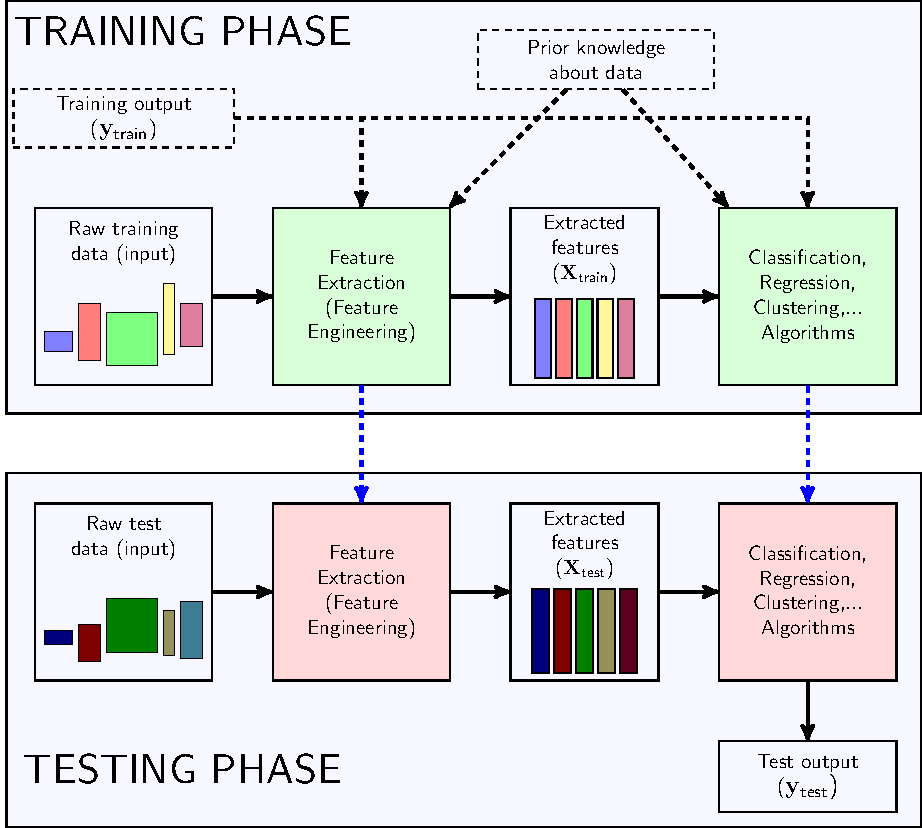
\includegraphics[width = \textwidth]{../FeatureEngineering/latex/ML_models.pdf}
   \caption{Mô hình chung cho các bài toán Machine Learning.}
   \label{fig:}
 \end{figure}
 
Có hai phases lớn là Training phase và Testing phase. Xin nhắc lại là với các bài toán Supervised learning, ta có các cặp dữ liệu (\textit{input, output}), với các bài toán Unsupervised learing, ta chỉ có \textit{input} mà thôi. 
  
 
\subsection{TRAINING PHASE }
Có hai khối có nền màu xanh lục chúng ta cần phải thiết kế:  
 
 
\subsubsection{Feature Extractor }
\textbf{ĐẦU RA} 
 
Tôi xin đề cập đầu ra của khối này trước vì mục đích của Feature Engineering là tạo ra một Feature Extractor biến dữ liệu thô ban đầu thành dữ liệu phù hợp với từng mục đích khác nhau.  
 
\textbf{ĐẦU VÀO} 
\begin{itemize}
    \item \textbf{\textit{raw training input}}. Raw input là tất cả các thông tin ta biết về dữ liệu. Ví dụ: với ảnh thì là giá trị của từng pixel; với văn bản thì là từng từ, từng câu; với file âm thanh thì nó là một đoạn tín hiệu; với cơ sở dữ liệu \href{http://machinelearningcoban.com/2017/01/08/knn/#bo-co-so-du-lieu-iris-iris-flower-dataset}{Iris} thì nó là độ dài các cánh hoa và đài hoa, ... Dữ liệu thô này thường không ở dạng vector, không có số chiều như nhau. Thậm chí có thể có số chiều như nhau nhưng số chiều quá lớn, như một bức ảnh màu 1000 pixel x 1000 pixel thì số \textit{elements} đã là $3 \times 10^6$ (3 vì ảnh màu thường có 3 channels: Red, Green, Blue). Đây là một con số quá lớn, không lợi cho lưu trữ và tính toán.  

    \item \textbf{(optional) \textit{output} của \textit{training set}}. Trong các bài toán Unsupervised learning, ta không biết \textit{output} nên hiển nhiên sẽ không có đầu vào này. Trong các bài toán Supervised learning, có khi dữ liệu này cũng không được sử dụng. Ví dụ: nếu \textit{raw input} đã có cùng số chiều rồi nhưng số chiều quá lớn,  ta muốn giảm số chiều của nó thì cách đơn giản nhất là \textit{chiếu} vector đó xuống một không gian có số chiều nhỏ hơn bằng cách lấy một ma trận ngẫu nhiên nhân với nó. Ma trận này thường là ma trận \textit{béo} (số hàng ít hơn số cột, tiếng Anh - fat matrices) để đảm bảo số chiều thu được nhỏ hơn số chiều ban đầu. Việc làm này mặc dù làm mất đi thông tin, trong nhiều trường hợp vẫn mang lại hiệu quả vì đã giảm được lượng tính toán ở phần sau. Đôi khi \textit{ma trận chiếu} không phải là ngẫu nhiên mà có thể được \textit{học} dựa trên toàn bộ \textit{raw input}, ta sẽ có bài toán tìm ma trận chiếu để lượng thông tin mất đi là ít nhất. Trong nhiều trường hợp, dữ liệu \textit{output} của \textit{training set} cũng được sử dụng để tạo ra Feature Extractor. Ví dụ: trong bài toán classification, ta không quan tâm nhiều đến việc mất thông tin hay không, ta chỉ quan tâm đến việc những thông tin còn lại có đặc trưng cho từng class hay không. Ví dụ, dữ liệu thô là các hình vuông và hình tam giác có màu đỏ và xanh. Trong bài toán phân loại đa giác, các output là \textit{tam giác} và \textit{vuông},  thì ta không quan tâm tới màu sắc mà chỉ quan tâm tới số cạnh của đa giác. Ngược lại, trong bài toán phân loại màu, các class là \textit{xanh} và \textit{đỏ}, ta không quan tâm tới số cạnh mà chỉ quan tâm đến màu sắc thôi.  

    \item \textbf{(optional) \textit{Prior knowledge about data}}: Đôi khi những giả thiết khác về dữ liệu cũng mang lại lợi ích. Ví dụ, trong bài toán classification, nếu ta biết dữ liệu là (gần như) \href{http://machinelearningcoban.com/2017/01/21/perceptron/#bai-toan-perceptron}{ \textit{linearly separable}} thì ta sẽ đi tìm một ma trận chiếu sao cho ở trong không gian mới, dữ liệu vẫn đảm bảo tính \textit{linearly separable}, việc này thuận tiện hơn cho phần classification vì các thuật toán linear, nhìn chung, đơn giản hơn.  
\end{itemize}
 
Sau khi \textit{học} được feature extractor thì ta cũng sẽ thu được \textit{extracted features} cho \textit{raw input data}. Những \textit{extracted features} này được dùng để huấn luyện các thuật toán Classification, Clustering, Regression,... ở phía sau. 
 
 
\subsubsection{Main Algorithms }
Khi có được \textit{extracted features} rồi, chúng ta sử dụng những thông tin này cùng với (optional) \textit{training output} và (optional) \textit{prior knowledge} để tạo ra các mô hình phù hợp, điều mà chúng ta đã làm ở những bài trước.  
 
\textbf{Chú ý:} Trong một số thuật toán cao cấp hơn, việc \textit{huấn luyện} feature extractor và main algorithm được thực hiện cùng lúc với nhau chứ không phải từng bước như trên.  
 
\textbf{Một điểm rất quan trọng: khi xây dựng bộ \textit{feature extractor} và \textit{main algorithms}, chúng ta không được sử dụng bất kỳ thông tin nào trong tập \textit{test data}. Ta phải giả sử rằng những thông tin trong \textit{test data} chưa được nhìn thấy bao giờ. Nếu sử dụng thêm thông tin về \textit{test data} thì rõ ràng ta đã \textit{ăn gian}! Tôi từng đánh giá các bài báo khoa học quốc tế, rất nhiều tác giả xây dựng mô hình dùng cả dữ liệu \textit{test data}, sau đó lại dùng chính mô hình đó để kiểm tra trên \textit{test data} đó. Việc \textit{ăn gian} này là lỗi rất nặng và hiển nhiên những bài báo đó bị từ chối (reject).} 
 
 
\subsection{TESTING PHASE }
Bước này đơn giản hơn nhiều. Với \textit{raw input} mới, ta sử dụng feature extractor đã tạo được ở trên (tất nhiên không được sử dụng \textit{output} của nó vì \textit{output} là cái ta đang đi tìm) để tạo ra feature vector tương ứng. Feature vector được đưa vào \textit{main algorithm} đã được học ở training phase để dự đoán \textit{output}.  
 
 
\section{Một số ví dụ về Feature Engineering}
 
\subsection{Trực tiếp lấy raw data }
Với bài toán phân loại chữ số viết tay trong bộ cơ sở dữ liệu \href{http://machinelearningcoban.com/2017/01/04/kmeans2/#bo-co-so-du-lieu-mnist}{MNIST}, mỗi bức ảnh có số chiều là 28 pixel x 28 pixel (tất nhiên việc \textit{crop} và chỉnh sửa mỗi bức ảnh đã được thực hiện từ trước rồi, đó đã là một phần của feature engineering rồi). Một cách đơn giản thường được dùng là \textit{kéo dài} ma trận 28x28 này để được 1 vector có số chiều 784. Trong cách này, các cột (hoặc hàng) của ma trận ảnh được đặt chồng lên (hoặc cạnh nhau) để được 1 vector dài. Vector dài này được trực tiếp sử dụng làm feature đưa vào các bộ classifier/clustering/regression/... Lúc này, giá trị của mỗi pixel ảnh được coi là một feature.  
 
Rõ ràng việc làm đơn giản này đã làm mất thông tin về \textit{không gian} (spatial information) giữa các điểm ảnh, tuy nhiên, trong nhiều trường hợp, nó vẫn mang lại kết quả khả quan.  
 
\subsection{Feature selection }
Giả sử rằng các điểm dữ liệu có số features khác nhau (do kích thước dữ liệu khác nhau hay do một số feature mà điểm dữ liệu này có nhưng điểm dữ liệu kia lại không thu thập được), và số lượng features là cực lớn. Chúng ta cần \textit{chọn} ra một số lượng nhỏ hơn các feature phù hợp với bài toán. \textit{Chọn thế nào} và \textit{thế nào là phù hợp} lại là một bài toán khác, tôi sẽ không bàn thêm ở đây. 
 
 
\subsection{Dimensionality reduction }
Một phương pháp nữa tôi đã đề cập đó là làm giảm số chiều của dữ liệu để giảm bộ nhớ và khối lượng tính toán. Việc giảm số chiều này có thể được thực hiện bằng nhiều cách, trong đó \textit{random projection} là cách đơn giản nhất. Tức chọn một \textit{ma trận chiếu} (projection matrix) ngẫu nhiên (ma trận béo) rồi nhân nó với từng điểm dữ liệu (giả sử dữ liệu ở dạng vector cột) để được các vector có số chiều thấp hơn. Lúc này, có thể ta không có tên gọi cho mỗi feature nữa vì các feature ở vector ban đầu đã được trộn lẫn với nhau theo một tỉ lệ nào đó rồi lưu và vector mới này. Mỗi thành phần của vector mới này được coi là một feature (không tên).  
 
Việc chọn một ma trận chiếu ngẫu nhiên đôi khi mang lại kết quả tệ không mong muốn vì thông tin bị mất đi quá nhiều. Một phương pháp được sử dụng nhiều để hạn chế lượng thông tin mất đi có tên là \href{https://en.wikipedia.org/wiki/Principal_component_analysis}{Principle Component Analysis} sẽ được tôi trình bày sau đây khoảng 1-2 tháng.  
 
\textbf{Chú ý:} Feature learning không nhất thiết phải làm giảm số chiều dữ liệu, đôi khi feature vector còn có số chiều lớn hơn raw data. Random projection cũng có thể làm được việc này nếu ma trận chiếu là một ma trận \textit{cao} (số cột ít hơn số hàng). 
 
 
\subsection{Bag-of-words }
Hẳn rất nhiều bạn đã tự đặt câu hỏi: Với một văn bản thì feature vector sẽ có dạng như thế nào? Làm sao đưa các từ, các câu, đoạn văn ở dạng \textit{text} trong các văn bản về một vector mà mỗi phần tử là một số?  
 
Có một phương pháp rất phổ biến giúp bạn trả lời những câu hỏi này. Phương pháp đó có tên là \textit{Bag of Words (BoW)} (\textit{Túi đựng Từ}). 
 
Vẫn theo thói quen, tôi bắt đầu bằng một ví dụ. Giả sử chúng ta có bài toán phân loại tin rác. Ta thấy rằng nếu một tin có chứa các từ \textit{khuyến mại, giảm giá, trúng thưởng, miễn phí, quà tặng, tri ân, ...} thì nhiều khả năng đó là một tin nhắn rác. Vậy phương pháp đơn giản nhất là \textit{đếm} xem trong tin đó có bao nhiêu từ thuộc vào các từ trên, nếu nhiều hơn 1 ngưỡng nào đó thì ta quyết định đó là tin rác. (Tất nhiên bài toán thực tế phức tạp hơn nhiều khi các từ có thể được viết dưới dạng không dấu, hoặc bị cố tình viết sai chính tả, hoặc dùng ngôn ngữ teen). Với các loại văn bản khác nhau thì lượng từ liên quan tới từng chủ đề cũng khác nhau. Từ đó có thể dựa vào số lượng các từ trong từng loại để làm các vector đặc trưng cho từng văn bản.  
 
Tôi xin lấy ví dụ cụ thể hơn về cách tạo ra vector đặc trưng cho mỗi văn bản dựa trên BoW và xin được lấy tiếng Anh làm ví dụ (nguồn \href{https://en.wikipedia.org/wiki/Bag-of-words_model}{Bag of Words wiki}. Tiếng Việt khó hơn vì một từ có thể có nhều âm tiết, tiếng Anh thì thường cứ gặp dấu cách là kết thúc một từ).  
 
Giả sử chúng ta có hai văn bản đơn giản: 
 
\begin{lstlisting}[language=Python]
(1) John likes to watch movies. Mary likes movies too. 
\end{lstlisting}
 
và  
 
\begin{lstlisting}[language=Python]
(2) John also likes to watch football games. 
\end{lstlisting}
Dựa trên hai văn bản này, ta có danh sách các từ được sử dụng, được gọi là \textit{từ điển} với 10 \textit{từ} như sau: 
 
\begin{lstlisting}[language=Python]
["John", "likes", "to", "watch", "movies", "also", "football", "games", "Mary", "too"] 
\end{lstlisting}
Với mỗi văn bản, ta sẽ tạo ra một vector đặc trưng có số chiều bằng 10, mỗi phần tử đại diện cho số từ tương ứng xuất hiện trong văn bản đó. Với hai văn bản trên, ta sẽ có hai vector đặc trưng là: 
 
\begin{lstlisting}[language=Python]
(1) [1, 2, 1, 1, 2, 0, 0, 0, 1, 1] 
(2) [1, 1, 1, 1, 0, 1, 1, 1, 0, 0] 
\end{lstlisting}
Văn bản (1) có 1 từ "John", 2 từ "likes", 0 từ "also", 0 từ "football", ... nên ta thu được vector tương ứng như trên.  
 
Có một vài điều cần lưu ý trong BoW: 
\begin{itemize}
    \item Với những ứng dụng thực tế, \textit{từ điền} có nhiều hơn 10 từ rất nhiều, có thể đến một trăm nghìn hoặc cả triệu, như vậy vector đặc trưng thu được sẽ rất \textit{dài}. Một văn bản chỉ có 1 câu, và 1 tiểu thuyết nghìn trang đều được biểu diễn bằng các vector có số chiều bằng 100 nghìn hoặc 1 triệu.

    \item Có rất nhiều từ trong từ điển không xuất hiện trong một văn bản. Như vậy các vector đặc trưng thu được thường có rất nhiều phần tử bằng 0. Các vector có nhiều phần tử bằng 0 được gọi là \textit{sparse vector} (sparse hiểu theo nghĩa là \textit{thưa thớt, rải rác}, tôi xin phép chỉ sử dụng khái niệm này bằng tiếng Anh). Để việc lưu trữ được hiệu quả hơn, ta không lưu cả vector đó mà chỉ lưu \textit{vị trí} của các phần tử khác 0 và \textit{giá trị} tương ứng. Lưu ý: nếu có hơn 50% số phần tử khác 0, việc làm này lại phản tác dụng! 

    \item Thi thoảng có những từ hiếm gặp không nằm trong từ điển, vậy ta sẽ làm gì? Một cách thường được dùng là \textit{mở rộng} vector đặc trưng thêm 1 phần tử, gọi là phẩn tử \pythoninline{<Unknown>}. Mọi từ không có trong từ điền đều được coi là \pythoninline{<Unknown>}. 

    \item Nghĩ kỹ một chút, những từ hiếm đôi khi lại mang những thông tin qua trọng nhất mà chỉ loại văn bản đó có. Đây là một nhược điểm của BoW. Có một phương pháp cải tiến khác giúp khắc phục nhược điểm này có tên là Term Frequency-Inverse Document Frequency (TF-IDF) dùng để xác định tầm quan trọng của một từ trong một văn bản dựa trên toàn bộ văn bản trong cơ sở dữ liệu (corpus). Bạn đọc muốn tìm hiểu thêm có thể xem \href{https://www.gitbook.com/book/lizrush/algorithms-for-webdevs-ebook/details}{5 Algorithms Every Web Developer Can Use and Understand, section 5.} 

    \item Nhược điểm lớn nhất của BoW là nó không mang thông tin về thứ tự của các từ. Cũng như sự liên kết giữa các câu, các đoạn văn trong văn bản. Ví dụ, ba câu sau đây: "Em yêu anh không?", "Em không yêu anh", và "Không, (nhưng) anh yêu em" khi được trích chọn đặc trưng bằng BoW sẽ cho ra ba vector giống hệt nhau, mặc dù ý nghĩa khác hẳn nhau. 
\end{itemize}
 
\textbf{Bonus:} hình dưới đay là tần suất sử dụng các từ (coi mỗi âm tiết là một từ) trong Truyện Kiều (\href{https://bitbucket.org/tiepvupsu/vietnamese/src/c6f3af6050f8ca911ed0fa209220ce3c99010075/TruyenKieu2.txt?at=master&fileviewer=file-view-default}{theo bản này}) nếu ta chỉ sử dụng 30 từ có tần suất cao nhất. : 
% <div class="imgcap"> 
% <img src ="\assets\FeatureEngineering\truyenkieu.png" align = "center" width = "400"> 
% <div class = "thecap">Hình 2: Bag of Words cho Truyện Kiều với 30 từ có tần suất cao nhất.</div> 
% </div>  
 
 
\subsection{Bag-of-Words trong Computer Vision }
Bags of Words cũng được áp dụng trong Computer Vision với cách định nghĩa \textit{words} và từ điển khác.  
 
Xét các ví dụ sau:  
 
\textbf{Ví dụ 1:} 
 
Có hai class ảnh, một class là ảnh các khu rừng, một class là ảnh các sa mạc. Phân loại một bức ảnh là rừng hay sa mạc (giả sử ta biết rằng nó thuộc một trong hai loại này) một cách trực quan nhất là dựa vào màu sắc. Màu xanh nhiều thì là rừng, màu đỏ và vàng nhiều thì là sa mạc. Vậy chúng ta có thể có một mô hình đơn giản để trích chọn đặc trưng như sau: 

\begin{itemize}
    \item Với một bức ảnh, chuẩn bị một vector $\mathbf{x}$ có số chiều bằng 3, đại diện cho 3 màu xanh ($x_1$), đỏ ($x_2$), và vàng ($x_3$).  

    \item Với mỗi điểm ảnh trong bức ảnh đó, xem nó gần với màu xanh, đỏ hay vàng nhất dựa trên giá trị của pixel đó. Nếu nó gần điểm xanh nhất, tăng $x_1$ lên 1; gần đỏ nhất, tăng $x_2$ lên 1; gần vàng nhất, tăng $x_3$ lên 1.  

    \item Sau khi xem xét tất cả các điểm ảnh, dù cho bức ảnh có kích thước thế nào, ta vẫn thu được một vector có độ dài bằng 3, mỗi phần tử thể hiện việc có bao nhiêu pixel trong bức ảnh có màu tương ứng. Vector cuối này còn được gọi là vector histogram của bức ảnh tương ứng với ba màu xanh, đỏ, vàng. Dựa vào vector này, ta có thể quyết định bức ảnh đó là ảnh rừng hay sa mạc.  
\end{itemize}
 
\textbf{Ví dụ 2:} 
 
Trên thực tế, các bài toán xử lý ảnh không đơn giản như ví dụ 1 trên đây. Mắt người thực ra nhạy với các đường nét, hình dáng hơn là màu sắc. Một cái (ảnh) cây dù không có màu vẫn là một cái (ảnh) cây! Vì vậy, xem xét giá trị từng điểm ảnh một không mang lại kết quả khả quan vì lượng thông tin bị mất quá nhiều.  
 
Có một cách khắc phục là thay vì xem xét một điểm ảnh, ta xem xét một \textit{cửa sổ} nhỏ trong ảnh (trong Computer Vision, cửa sổ này được gọi là patch) là một hình chữ nhật chứa nhiều điểm ảnh gần nhau. Cửa sổ này đủ lớn để có thể chứa được các bộ phận có thể mô tả được vật thể trong ảnh.  
 
Ví dụ với mặt người, các patch nên đủ lớn để chứa được các phần của khuôn mặt như mắt, mũi, miệng như hình dưới đây.  
 
% <div class="imgcap"> 
% <img src ="\assets\FeatureEngineering\bow_face.png" align = "center" width = "800"> 
% <div class = "thecap">Hình 3: Bag of Words cho ảnh chứa mặt người. (Nguồn <a href="http://www.robots.ox.ac.uk/~az/icvss08_az_bow.pdf"> Bag of visual words model: recognizing object categories</a>)</div> 
% </div>  
 
Tương tự thế, với ảnh là ô tô, các patch thu được có thể là bánh xe, khung xe, cửa xe, ... như hàng trên trong hình dưới đây.  
 
% <div class="imgcap"> 
% <img src ="\assets\FeatureEngineering\bow_car.png" align = "center" width = "800"> 
% <div class = "thecap">Hình 4: Bag of Words cho ảnh ô tô. (Nguồn: tôi cố gắng tìm nguồn cho hình này nhưng tất cả các tài liệu tôi tìm được đều ghi "Source: B. Leibe", tôi cũng xin được trích nguồn tương tự)</div> 
% </div>  
 
Có một câu hỏi đặt ra là, trong xử lý văn bản, hai từ được coi là như nhau nếu nó được biểu diễn bởi các ký tự giống nau. Vậy trong xử lý ảnh, hai patchés được coi là như nhau khi nào? Khi mọi pixel trong hai patches có giá trị bằng nhau sao?  
 
Câu trả lời là không. Xác suất để hai patches giống hệt nhau từng pixel là rất thấp vì có thể một phần của vật thể trong một patch bị lệch đi vài pixel so với phần đó trong patch kia; hoặc phần vật thể trong patch bị méo, hoặc có độ sáng khác nhau, mặc dù ta vẫn nhìn thấy hai patches đó \textit{rất giống nhau}. Vậy thì hai patch được coi là như nhau khi nào? Và \textit{từ điển} ở đây được định nghĩa như thế nào?  
 
Câu trả lời ngắn: hai patches là gần giống nhau nếu khoảng cách Euclid giữa hai vector tạo bởi hai patches đó gần nhau. Từ điển (codebook) sẽ có số phần tử do ta tự chọn. Số phần tử càng cao thì độ sai lệch càng ít, nhưng sẽ nặng về tính toán hơn.  
 
Câu trả lời dài: chúng ta có thể áp dụng \href{http://machinelearningcoban.com/2017/01/01/kmeans/}{K-means clustering}. Với rất nhiều patches thu được, giả sử ta muốn xây dựng một \textit{codebook} với chỉ khoảng 1000 \textit{words}. Vậy thì ta cho $k = 1000$ rồi thực hiện K-means clustering trên toàn bộ số patches thu được (từ tập training). Sau khi thực hiện K-means clustering, ta thu được 1000 clusters và 1000 centers tương ứng. Mỗi centers này được coi là một \textit{words}, và tất cả những điểm rơi vào cùng một cluster được coi là cùng một bag. Với ảnh trong tập test data, ta cũng lấy các patches rồi xem chúng rơi vào những bags nào. Từ đó suy ra vector đặc trưng cho mỗi bức ảnh. Chú ý rằng với $k = 1000$, mỗi bức ảnh sẽ được \textit{mô tả} bởi một vector có số chiều 1000, tức là mỗi điểm dữ liệu bây giờ đã có số chiều bằng nhau, mặc dù ảnh thô đầu vào có thể có kích thước khác nhau. 
 
\subsection{Feature Scaling and Normalization}
(Tham khảo \href{https://en.wikipedia.org/wiki/Feature_scaling}{Feature Scaling wiki}). 
 
Các điểm dữ liệu đôi khi được đo đạc với những đơn vị khác nhau, m và feet chẳng hạn. Hoặc có hai thành phần (của vector dữ liệu) chênh lệch nhau quá lớn, một thành phần có khoảng giá trị từ 0 đến 1000, thành phần kia chỉ có khoảng giá trị từ 0 đến 1 chẳng hạn. Lúc này, chúng ta cần chuẩn hóa dữ liệu trước khi thực hiện các bước tiếp theo.  
 
\textbf{Chú ý:} việc chuẩn hóa này chỉ được thực hiện khi vector dữ liệu đã có cùng chiều. 
 
Một vài phương pháp chuẩn hóa thường dùng: 
 
\subsubsection{Rescaling }
Phương pháp đơn giản nhất là đưa tất cả các thành phần về cùng một khoảng, $[0, 1]$ hoặc $[-1, 1]$ chẳng hạn, tùy thuộc vào ứng dụng. Nếu muốn đưa một thành phần (feature) về khoảng $[0, 1]$, công thức sẽ là:  
\begin{equation*} 
x' = \frac{x - \min(x)}{\max(x) - \min(x)} 
\end{equation*} 
trong đó $x$ là giá trị ban đầu, $x'$ là giá trị sau khi chuẩn hóa. $\min(x), \max(x)$ được tính trên toàn bộ dữ liệu training data ở cùng một thành phần. Việc này được thực hiện trên từng thành phần của vector dữ liệu $\mathbf{x}$.  
 
 
\subsubsection{Standardization }
Một phương pháp nữa cũng hay được sử dụng là giả sử mỗi thành phần đều có phân phối chuẩn với kỳ vọng là 0 và phương sai là 1. Khi đó, công thức chuẩn hóa sẽ là:  
\begin{equation*} 
x' = \frac{x - \bar{x}}{\sigma} 
\end{equation*} 
với $\bar{x}, \sigma$ lần lượt là kỳ vọng và phương sai (standard deviation) của thành phần đó trên toàn bộ training data.  
 
\subsubsection{Scaling to unit length }
Một lựa chọn khác nữa cũng được sử dụng rộng rãi là chuẩn hóa các thành phần của mỗi vector dữ liệu sao cho toàn bộ vector có độ lớn (Ecluid, tức \href{http://machinelearningcoban.com/math/#norm2}{norm 2}) bằng 1. Việc này có thể được thực hiện bằng: 
\begin{equation*} 
\mathbf{x}' = \frac{\mathbf{x}}{\|\mathbf{x}\|_2} 
\end{equation*} 
 
 
\section{Thảo luận}
Xem ra thế giới Machine Learning rất rộng lớn và có rất nhiều thứ chúng ta cần làm. Và 
vẫn có khá nhiều thứ tôi có thể viết được. Tuy nhiên, blog này sẽ không tập trung nhiều vào Feature Learning, mặc dù sẽ có một vài bài nói về Dimensionality Reduction. Tôi sẽ sử dụng các bộ dữ liệu có sẵn, và đã qua bước Feature Learning.  
 
 
\section{Tài liệu tham khảo }
[1] \href{https://en.wikipedia.org/wiki/Feature_engineering}{Feature Enginieering - wiki} 

[2] \href{https://en.wikipedia.org/wiki/Feature_scaling}{Feature Scaling wiki} 

[3] Csurka, Gabriella, et al. "\href{https://people.eecs.berkeley.edu/~efros/courses/AP06/Papers/csurka-eccv-04.pdf}{Visual categorization with bags of keypoints.}" Workshop on statistical learning in computer vision, ECCV. Vol. 1. No. 1-22. 2004.  

[4] \href{https://en.wikipedia.org/wiki/Bag-of-words_model}{Bag of Words model - wiki} 

[5] \href{https://www.kaggle.com/c/word2vec-nlp-tutorial/details/part-1-for-beginners-bag-of-words}{Bag of Words Meets Bags of Popcorn} 
 
